\chapter{The LTLCreator prototype}
\label{chap:theltlcreatorprototype}

As stated in chapter~\ref{chap:goals}, appropriate support by a graphical editor is important for the usefulness of the developed visual language. Therefore a prototype of such an editor has been designed and implemented which contains the visual language as well as the proposed constraint generation heuristics. The implementation is a Java Swing component and has a simple API definition, making it easy to integrate the \emph{LTLCreator} tool into other java applications.

First of all the model implementation for representing state machines is described in section~\ref{sec:statemachinemodel}. Then, some details about the implementation of the visual language are given in section~\ref{sec:prototype:operatorconstraints}, directly followed by an explanation about the realization of the automated constraint generation functionality in section~\ref{sec:prototype:automatedconstraintgeneration}.
The assembly of all the previous features in one tool is described in section~\ref{sec:coalescence}. However, the tool's functionality shall also be available in Robostudio in order to provide safety mechanisms for the healthcare service robots and to be a prototype for evaluation. Section~\ref{sec:integrationintorobostudio} gives a main idea how an integration into Robostudio is possible. 


\section{State machine model}
\label{sec:statemachinemodel}

For the checking of constraints as well as for the constraint generation a model is needed which represents the state machine program. Three classes are responsible for holding the state machine program with all its necessary information: The class \emph{Fsm} represents the finite state machine and lists all contained states. It is called finite state machine, because the number of states is finite which applies to the domain of this work. \emph{State} represents the states of the machine and holds all transitions from and to the respective state. Transitions are represented by the class \emph{Transition} which specifies the source and a target state. Figure~\ref{fig:fsm_class} shows all three class definitions for the state machine model.

\begin{figure}[htbp]
  \centering
  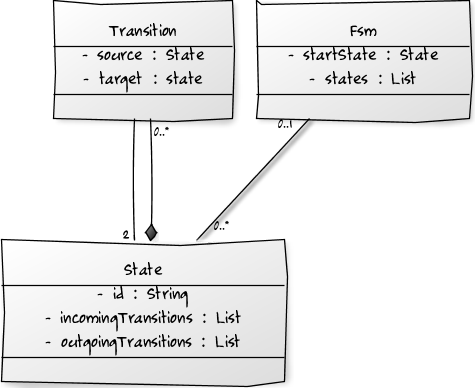
\includegraphics[width=0.65\linewidth]{fsm_class} 
  \caption{Class definitons for the state machine model.}
  \label{fig:fsm_class}
\end{figure}




\section{Operator constraints}
\label{sec:prototype:operatorconstraints}

All operator types, i.e. \emph{IfThenOperator}, \emph{AndOperator}, \emph{OrOperator}, \emph{NotOperator}, \emph{NextOperator}, \emph{FutureOperator}, \emph{AlwaysOperator}, \emph{UntilOperator} and \emph{StateOperator}, are realized by dedicated classes. All of them inherit from one abstract class \emph{AbstractOperator} which provides the basic functionality beeing used by all operators. The \emph{AbstractOperator} class is shown in figure~\ref{fig:abstractoperator} and its methods are described as follows:

\begin{description}
	\item[getLTL():] This function returns the LTL formula of an operator and all its children recursively. Applied to the most outer operator it returns the complete formula for the constraint. This function is abstract and implemented by each operator type separately.
	\item[getColor():] Each operator type has got is own significant color which can be retrieved by the abstract function \emph{getColor()}.
	\item[createNewInstance():] In order to provide operator creation over a tool bar, this function instantiates a new operator object, depending on the implementation.
	%\item[setMouseOver(boolean):] Mouse over actions cause the underlying operator to be highlighted. This function makes all operators except the hovered one appearing bleeched out.
	%\item[paintOperator(Graphics, ...):] Each operator class has to implement the abstract function \emph{paintOperator()}. It manages all color and shape painting for the respective operator. Additional parameters such as recursive painting including children can be specified.
	%\item[contains(int, int):] Given two coordinates x and y, it can be determined whether the herewith defined point lays within an operator.
	\item[isSimilar(AbstractOperator):] Two operators can be compared for semantic equality. Equality is given if the compared operators are of the same type and similarly their children. This functionality is important for avoiding duplicate constraints during constraint generation, for example.
	\item[addChangeListener(OperatorChangeListener):] Whenever there is a change to the operator or to one of its children, an operator change listener gets notified about it. The hierarchical architecture of \emph{AbstractOperator}s propagates all change events to the root operator. The function \emph{addChangeListener()} allows registering for such change notifications.
	\item[removeChangeListener(OperatorChangeListener):] According to \emph{addChangeListener} this function allows deregistration again.
\end{description}

\begin{figure}[htbp]
  \centering
  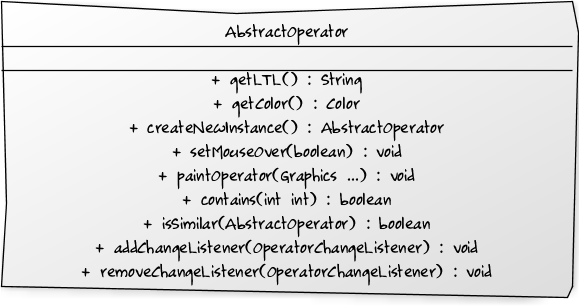
\includegraphics[width=0.6\linewidth]{AbstractOperator} 
  \caption{Class definition for \emph{AbstractOperator}.}
  \label{fig:abstractoperator}
\end{figure}

Whereas \emph{StateOperator}s have no operator children and are leafs in the syntax tree of LTL formulas, all other operator types are either unary or binary operators with one or two optional nested children respectively. 
The graphical representation of both unary and binary operators thus needs to have place holders and docking stations
\begin{wrapfigure}{r}{0.40\textwidth}
  \centering
  
\includegraphics[scale=0.65]{bucket_example.jpg}
  \caption{Buckets for graphical nesting of operators.}
  \label{fig:bucket_example}
\end{wrapfigure}
for sub operators. These are realized by buckets which display a small ``drop'' label as shown in figure~\ref{fig:bucket_example} and allow operator adding or removing by mouse drops.
For this a class \emph{Bucket} is defined with get and set methods for defining a sub operator.
Figure~\ref{fig:klassendiagramm_operators} depicts the relationship between \emph{AbstractOperator}, \emph{Bucket} and operator implementations.
Once operators are composed in a way that no empty buckets are left over, a complete constraint such as the one shown in figure~\ref{fig:operator_tree} is retrieved. This diagram illustrates the correlation of nested operators and buckets.
\begin{figure}[htbp]
  \centering
  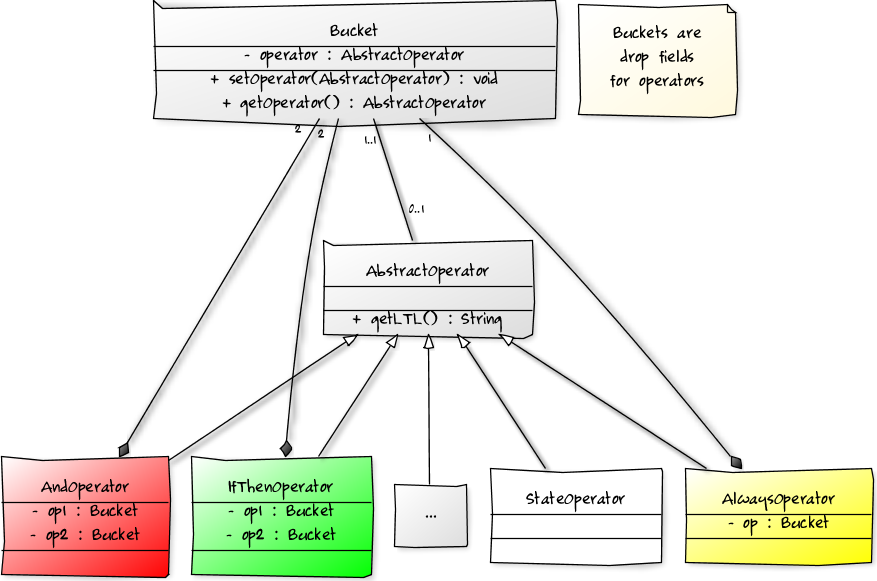
\includegraphics[width=\linewidth]{klassendiagramm_operators} 
  \caption{Class diagram of operator structure.}
  \label{fig:klassendiagramm_operators}
\end{figure}

\begin{figure}[htbp]
  \centering
  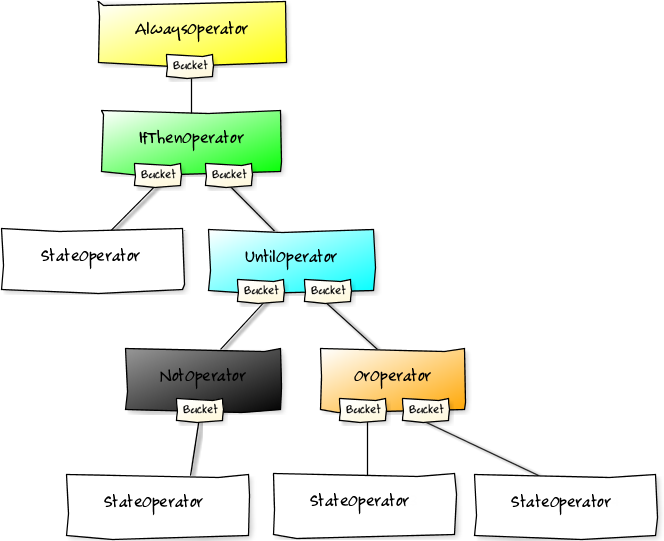
\includegraphics[width=0.95\linewidth]{operator_tree} 
  \caption{Instantiation of a constraint with several operators.}
  \label{fig:operator_tree}
\end{figure}

For the prototype implementation, all graphical components such as buckets and operators are implemented as Java Swing \emph{JComponent}. Thereby a lot of functionality for the visual configuration is already available such as the complex layout and repaint concept and the container functionality which is used for unary and binary operators as well as buckets.

%PAINT

Swing allows the implementation of a \emph{paint()} method which is responsible for rendering the component. This is used for giving every operator its special look. Swing's \emph{Graphics2D} functionality provides a great support in painting rounded shapes and color gradients. An operator is displayed as a rounded rectangle with dents around sub operators; it is displayed with a flowing backgound and borders and labels in the operator type's specific color. For the significant shape multiple rounded rectangles with and without borders are arranged in a way that the result appears to be one piece. Figure~\ref{fig:paintprocess} demonstrates how the process of painting works: For painting the \emph{IfThenOperator}, first of all a blank rectangle with border is drawn, directly followed by two filled rectangles with border which are placed where the two child operators shall be later on. In the third step the same rectangle as from step one is painted on top, this time without border. This makes all crossing borders disappear. Only labels and buckets still have to be added to create a complete \emph{IfThenOperator}.

\begin{figure}[htbp]
  \centering
  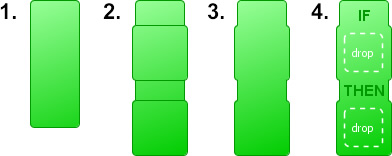
\includegraphics[scale=0.65]{paintprocess} 
  \caption{Four steps of painting an operator.}
  \label{fig:paintprocess}
\end{figure}

%LAYOUT

As proposed in the requirements for the visual language in section~\ref{sec:operatorconstraintformalism}, constraints have particular meanings for the two dimensions: A vertical read direction and the horizontal direction for variation in time. 
Swing's mechanism for layouting components is used for the positioning of operators. After determining the aspired sizes of child components which represent sub operators, reference lines which have been already demonstrated with figure~\ref{fig:referencelines} in section~\ref{sec:operatorconstraintformalism} are computed mathematically. Based on this information operators are sized and positioned correctly.

%MOUSE OVER

Regarding to the requirement for simple reading of constraints based on mouse hovering, the editor prototype supports context sensitive highlighting of particular constraint parts.
The built-in mouse support of Swing is used for identifying the operator positioned under the mouse cursor. All operators except the hovered one and its sub operators are presented bleached out which causes the hovered operator to appear emphasized. The most right operator composition in figure~\ref{fig:nested_and_mouseover} gives a demonstration of this idea.

%PROBLEM WITH MOUSE OVER AND MERGING

However, the concept of operator highlighting causes trouble in combination with the graphical merging of visual operators which was introduced in section~\ref{sec:designdecisions}. Since a merged operator does not have its own border, it can not be displayed as desired when hovered. This fact is also a problem for the editing: The graphical presentation does not support changing of merged operators, because it seems that they can not be picked by the mouse.
In order to retain full editability, hovered operators are excluded from the merge rule and still have to be displayed separated (see~figure~\ref{fig:nested_and_mouseover}).
\begin{figure}[htbp]
  \centering
  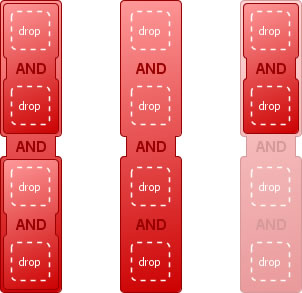
\includegraphics[scale=0.65]{and_simplify_mouseover}
  \caption{Default nested \emph{AND} operator, visually merged nested \emph{AND} operator and visually nested \emph{AND} operator with mouse over (from left to right).
  }
  \label{fig:nested_and_mouseover}
\end{figure}

%DRAG&DROP

Besides its importance for mouse hovering, Swing's mouse support is also used for determining the position where operators have to be added after drag and drop edit actions. So far
% the predefined Swing drag and drop has not been used but
a simple drag and drop mechanism called \emph{DndHandler} has been implemented whose class structure is shown in figure~\ref{fig:dndclassstructure}.
\begin{figure}[htbp]
  \centering
  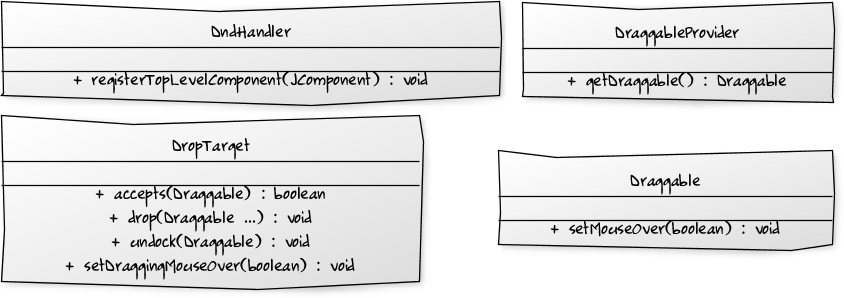
\includegraphics[width=\linewidth]{dndclassstructure} 
  \caption{Class definition for drag and drop functionality.}
  \label{fig:dndclassstructure}
\end{figure}% instead. 
Once a \emph{JComponent} is registered to the \emph{DndHandler}, it automatically manages any drag and drop actions with \emph{JComponent}s which implement either the \emph{Draggable} or \emph{DropTarget} interface. The former is implemented by all operators and specifies that this object can be moved from and to buckets or the dashboard, the latter is implemented by buckets and the dashboard and determines that it can accept and contain \emph{Draggable}s such as operators.
%Figure~\ref{fig:dndclassstructure} gives a short class overview.
Furthermore there is a class \emph{DraggableProvider} which is similar to \emph{Draggable} except that it is not moved itself but creates a new instance of the respective \emph{Draggable} implementation type which is then moved instead.

%TOOLBAR

\emph{LTLCreator} is equipped with a tool bar which provides all functionalities needed for constraint editing: For each operator type a \emph{DraggableProvider} is displayed as an icon in the respective operator color. Each time the mouse is pressed on it (drag action start), a new instance of the respective operator type is created which can be moved and dropped to the dashboard. Additionally, a trash can icon is displayed within the tool bar. It implements the \emph{DropTarget} interface and can thus receive operators. Its purpose is to provide a remove functionality for already instantiated operators which are not needed anymore.









\section{Automated constraint generation}
\label{sec:prototype:automatedconstraintgeneration}

As stated in section~\ref{sec:subgraphdefinition}, the automated generation of constraints for a state machine is based on subgraphs. For the finding of such subgraphs an algorithm has been developed. Section~\ref{sec:subgraphfindingconcept} aims to explain the basic concept of the algorithm, section~\ref{sec:subgraphfindingimplementation} introduces the slightly modified algorithm which is used for the prototype.
%It is described as follows:


\subsection{Subgraph finding concept}
\label{sec:subgraphfindingconcept}

First of all a start state ($\alpha$) is defined which has two or more outgoing transitions. All possible paths are generated which start from it and lead through the state machine. Every path ends before it visits states twice.
The result is a finite set of finite paths since loops are eliminated. Now every state gets as label assigned a number which represents the total number of occurrences of this state in all collected paths. In other words, the label of a state expresses the number of paths which start in the $\alpha$-state and contain this state. The $\alpha$-state itself is labeled with the total number of paths. If during walking through any of the paths a second state can be found with the same label, it means that all paths starting at $\alpha$-state come all together in this state again. It is determined to be a potential corresponding end state ($\beta$).
A last check has to be applied whether there are incoming transitions from outside into the subgraph which do not originally come from $\alpha$-state. If no such transitions are detected, a subgraph is found.
If there is no state with the same label, or a transition exists which comes from outside, the state machine as a whole can be assumed as subgraph beginning with $\alpha$-state insofar as the state machine does not contain further loops or terminating end states. Figure~\ref{fig:subgraph_finding} illustrates this concept of subgraph finding and shows all possible paths as well as the number of occurrences of each state.
\begin{figure}[htbp]
  \centering
  
  \tikzstyle{state} = [circle,fill=white,draw]
  \tikzstyle{statein} = [circle,fill=blue!20,draw]
  \tikzstyle{none} = [fill=white]
  \tikzstyle{highlighted} = [fill=yellow]
  \tikzstyle{every path} = [font=\sffamily\small]
  
	\begin{tikzpicture}[->,>=stealth',shorten >=1pt,auto,node distance=15mm]
	
	  \node[state] (1) at (0,0) {A};
	  \node[state] (4) [below left of=1] {B};
	  \node[state] (6) [below of=4] {D};
	  \node[state] (7) [below right of=4] {E};
	  \node[state] (5) [below right of=1] {C};
	  \node[state] (8) [below of=5] {F};
	  \node[state] (9) [below of=7] {G};
	  \node[state] (11) [below left of=9] {H};
	  \node[state] (12) [right of=9] {I};
	  
	  \node[state] (101) at (3,0) {A};
	  \node[state] (102) [below of=101] {B};
	  \node[state] (103) [below of=102] {D};
	  \node[state] (104) [below of=103] {G};
	  \node[state] (105) [below of=104] {H};
	  
	  \node[state] (201) at (4.5,0) {A};
	  \node[state] (202) [below of=201] {B};
	  \node[state] (203) [below of=202] {D};
	  \node[state] (204) [below of=203] {G};
	  \node[state] (205) [below of=204] {I};
	  
	  \node[state] (301) at (6,0) {A};
	  \node[state] (302) [below of=301] {B};
	  \node[state] (303) [below of=302] {E};
	  \node[state] (304) [below of=303] {G};
	  \node[state] (305) [below of=304] {H};
	  
	  \node[state] (401) at (7.5,0) {A};
	  \node[state] (402) [below of=401] {B};
	  \node[state] (403) [below of=402] {E};
	  \node[state] (404) [below of=403] {G};
	  \node[state] (405) [below of=404] {I};
	 
	  \node[state] (501) at (9,0) {A};
	  \node[state] (502) [below of=501] {C};
	  \node[state] (503) [below of=502] {F};
	  \node[state] (504) [below of=503] {G};
	  \node[state] (505) [below of=504] {H};
	  
	  \node[state] (601) at (10.5,0) {A};
	  \node[state] (602) [below of=601] {C};
	  \node[state] (603) [below of=602] {F};
	  \node[state] (604) [below of=603] {G};
	  \node[state] (605) [below of=604] {I};
	 
	  \node[highlighted] (701) at (12,0) {A=6};
	  \node[none] (702) at (12,-0.6) {B=4};
	  \node[none] (703) at (12,-1.2) {C=2};
	  \node[none] (703) at (12,-1.8) {D=2};
	  \node[none] (703) at (12,-2.4) {E=2};
	  \node[none] (703) at (12,-3.0) {F=2};
	  \node[highlighted] (703) at (12,-3.6) {G=6};
	  \node[none] (703) at (12,-4.2) {H=3};
	  \node[none] (703) at (12,-4.8) {I=3};
	  
		%\draw[->] (0, 0) .. controls(1,1) .. (3, 0);
		\draw[->] (12) to [out=45, in=0] (1);
	
	  \path[]
	  	(1) edge node [left] {} (4)
	        edge node [left] {} (5)
	    (4) edge node [left] {} (6)
	        edge node [left] {} (7)
	    (5) edge node [left] {} (8)
	    (6) edge node [left] {} (9)
	    (7) edge node [left] {} (9)
	    (8) edge node [left] {} (9)
	    (11) edge [bend left] node [left] {} (9)
	    (9) edge [bend left] node [left] {} (11)
	    (9) edge node [left] {} (12)
		  
		  
		  (101) edge node [left] {} (102)
		  (102) edge node [left] {} (103)
		  (103) edge node [left] {} (104)
		  (104) edge node [left] {} (105)
		  
		  (201) edge node [left] {} (202)
		  (202) edge node [left] {} (203)
		  (203) edge node [left] {} (204)
		  (204) edge node [left] {} (205)
		  
		  (301) edge node [left] {} (302)
		  (302) edge node [left] {} (303)
		  (303) edge node [left] {} (304)
		  (304) edge node [left] {} (305)
		  
		  (401) edge node [left] {} (402)
		  (402) edge node [left] {} (403)
		  (403) edge node [left] {} (404)
		  (404) edge node [left] {} (405)
		  
		  (501) edge node [left] {} (502)
		  (502) edge node [left] {} (503)
		  (503) edge node [left] {} (504)
		  (504) edge node [left] {} (505)
		  
		  (601) edge node [left] {} (602)
		  (602) edge node [left] {} (603)
		  (603) edge node [left] {} (604)
		  (604) edge node [left] {} (605)
		  ;
	
	\end{tikzpicture}
  \caption{Example for the subgraph finding algorithm: The occurrence labels of the states lead to
   %of each state in the paths lets you determine 
   G as an end state ($\beta$) corresponding to A.}
  \label{fig:subgraph_finding}
\end{figure}
This procedure is suitable for checking whether a state is the beginning of a subgraph and for discovering the corresponding $\beta$-state. In order to detect all subgraphs within a state machine, this procedure has to be applied to every single state which has two or more outgoing transitions. In order to improve the further finding of subgraphs and walking through the state machine, all already found subgraphs can be assumed as single states since it is already known where their paths come finally together again.%: In their $\beta$-states.



\subsection{Subgraph finding implementation}
\label{sec:subgraphfindingimplementation}

Following the previous description an algorithm has been implemented in Java. Its realization differs from the presented concept: Paths are not listed but states are directly labelled since not saving all possible paths is more memory efficient.
The state machine is traversed similarly to a depth-first search and each visited state's label is incremented by one. If the current state holds more than one outgoing transition and thus constitutes new paths,  all states on the current stack, i.e. the previously visited states on the current path, get their labels incremented by ('number of outgoing transitions' - 1). The algorithm turns back whenever it comes across a state which has already been visited within the same path stack of the depth-first search.

The overall implemented way of subgraph finding is illustrated in pseudo code with algorithm~\ref{alg:subgraphfinding}.
\begin{algorithm}
\caption{Finding of all subgraphs.}
\label{alg:subgraphfinding}
\begin{algorithmic}[1]
\STATE $subgraphs$: List
\FORALL{states as $S$}
  \STATE $start \leftarrow S$
	\STATE doLabelling($start$);
	\IF{state $E$ exists with label($E$)$=$label($S$)}
		\STATE $end \leftarrow E$
	\ELSE
		\STATE $end \leftarrow start$
	\ENDIF
	\IF{noCycles($start$, $end$) $and$ noExtTransitions($start$, $end$)}
		\STATE $subgraphs$.add($start$, $end$);
	\ENDIF
\ENDFOR
\end{algorithmic}
\end{algorithm}
Line 1 defines a variable $subgraphs$ which will contain all results of the algorithm after execution.
In line 4 the labelling process described above is executed by using one particular start state. Line 5 checks whether there is a state having the same label as the start state. If so, it is assumed as potential end state (line 6). Otherwise, the entire state machine is assumed to be a subgraph and the start state is defined as end state as well (line 8). Subsequent checks in line 9 finally determine whether it can be considered as proper subgraph.
There are no cycles allowed between start and end state since they are forbidden by the subgraph definition in section~\ref{sec:subgraphdefinition}.
Furthermore also foreign transitions are prohibited: Transitions coming from a state outside the subgraph are allowed to lead to the start state but not to other states of the subgraph. If all checks are successful, start and end states get added to the result list $subgraphs$ in line 11. This procedure is applied to all states of the state machine by the surrounding foreach loop (line 2). In the end, the list $subgraphs$ contains all pairs of start and end states which form subgraphs.


\subsection{Constraint generation}

After determining a subgraph, constraints are derived from it as defined in section~\ref{sec:constraintdetermination}. The entire process of constraint generation is illustrated by figure~\ref{fig:processofconstraintgeneration}.
\begin{figure}
  \centering

  \begin{sequencediagram}
		\tikzstyle{inststyle}+=[top color=yellow!30,bottom
color=white]
		\newthread{u}{User/Editor}{blue}
		\newthread[2.6]{cc}{Constraint creator}{red}
		\newinst[1]{alg}{Subgraph finding algorithm}

		\mess{u}{start(stm)}{cc}
		\begin{call}[3]{cc}{start(stm)}{alg}{finish}
			\begin{sdblock}[yellow!20]{For each subgraph}{}
				\setthreadbias{east}
				\begin{call}[3]{alg}{newSubgraph(subgraph)}{cc}{}
					\begin{sdblock}[yellow!20]{For each constraint}{}
						\begin{call}[3]{cc}{newConstraint(constraint)}{u}{}
						\end{call}
					\end{sdblock}
				\end{call}
				\setthreadbias{center}
			\end{sdblock}
		\end{call}
		\mess{cc}{finish}{u}
	\end{sequencediagram}
  
  \caption{Process of constraint generation.}
  \label{fig:processofconstraintgeneration}
\end{figure}
Once the user triggers the constraint generation for a state machine (stm), the subgraph finding algorithm starts working. When a subgraph is found, constraints are created and passed to the user. For each subgraph multiple constraint types can apply. This procedure is done iterative for each subgraph found.



The runtime of the algorithm depends on size and grade of branching of the state machine. An estimation about the execution time is presented later in section~\ref{sec:performance}. In order to improve waiting times and thus user experience during constraint generation the entire result might not be returned after termination but each subgraph should be processed as soon as it is found.
For this, the implementation for the algorithm has been extended by code snippets which frequently interact with so called \emph{ResultListener}s (figure~\ref{fig:resultlistener_class}).
%This interface is also implemented by the progress dialog.
An implementation of \emph{ResultListener} has to provide three methods which allow the algorithm to publish the current progress by calling \emph{void setProgress(int)} or to notify about newly found subgraphs by invoking \emph{void newSubGraphFound(SubGraph)}. The method \emph{boolean continueGeneration()} is called frequently and the execution will terminate as soon as it returns false.
\begin{figure}[htbp]
  \centering
  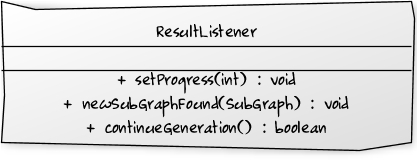
\includegraphics[width=0.50\linewidth]{resultlistener_class} 
  \caption{Interface definition of \emph{ResultListener}.}
  \label{fig:resultlistener_class}
\end{figure}

As a second approach aiming for better user experience during constraint generation, a dialog has been implemented which informs the developer continuously about the current progress. This includes the number of constraints found so far and a progress bar which gives a percentual estimation of execution time. Furthermore a cancel button permits premature stopping of the execution. A snapshot of the Dialog is shown in figure~\ref{fig:progressdialog}.
\begin{figure}[htbp]
  \centering
  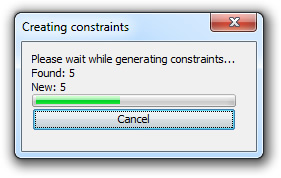
\includegraphics[width=0.34\linewidth]{progressdialog} 
  \caption{Snapshot of the progress dialog displayed during constraint generation.}
  \label{fig:progressdialog}
\end{figure}





\section{The LTLCreator}
\label{sec:coalescence}

Both features, the editor for the visual language presented in section~\ref{sec:operatorconstraintformalism} and the automated constraint generation in chapter~\ref{chap:automatedgenerationofsafetyconstraints}, were assembled in one tool, the \emph{LTLCreator}.
Figure~\ref{fig:LTLCreator} shows the assembled parts of LTLCreator: A dashboard is provided where constraints can be edited visually by the developer and result displays indicate the validation results of constraints graphically. For validating the constraints an external model checker is linked to \emph{LTLCreator}. This component does not have an UI as well as the constraint generator, which is also part of \emph{LTLCreator}. 
\begin{figure}[htbp]
  \centering
  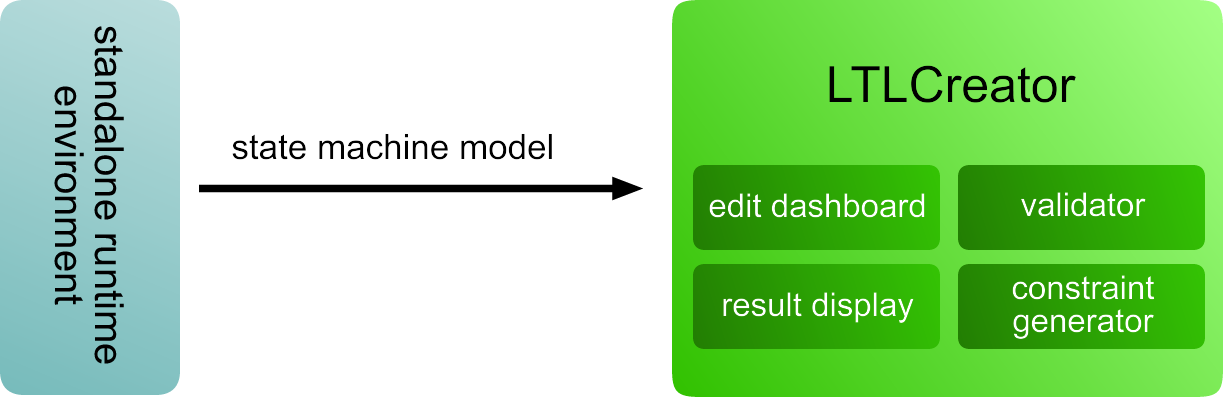
\includegraphics[width=0.65\linewidth]{LTLCreator}
  \caption{Integration of LTLCreator.}
  \label{fig:LTLCreator}
\end{figure}
The \emph{LTLCreator} itself does not provide functionalities for editing state machines although a state machine model is needed for the visual language as well as for constraint generation. Therefore the standalone version of \emph{LTLCreator} uses a hard coded state machine as model which represents an example program for test purpose.

Figure~\ref{fig:editor} shows a snapshot of the editor's environment:
\begin{figure}[htbp]
  \centering
  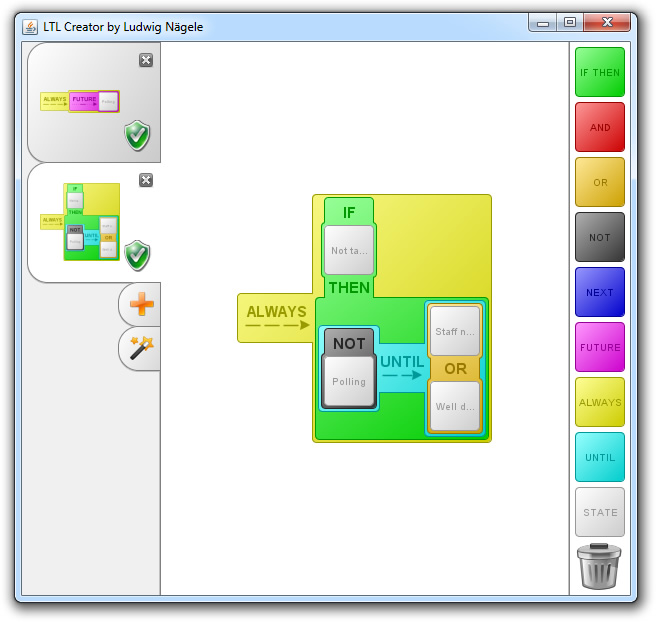
\includegraphics[width=\linewidth]{editor} 
  \caption{Snapshot of the visual editor LTLCreator.}
  \label{fig:editor}
\end{figure}
All functionalities needed for constraint editing are provided in the tool bar on the right (1). It contains draggable elements for creating all operator and proposition types as well as a trash can for deleting. Constraints can be composed by drag\&drop in the dashboard in the center of the editor (2) which holds and displays the operator constraints. The tab functionality on the left allows multiple constraints to be managed (3). Each tab shows a small thumbnail of the constraint and a symbol indicating its current status of validation result: For syntactically invalid constraints, an ``incomplete'' sign is displayed. Otherwise, an animated ring indicates that validation is in pro\-gress and will finally result in either a ``valid'' or ``invalid'' sign as shown in figure~\ref{fig:results}.
\begin{figure}[htbp]
  \centering
  
\includegraphics[scale=0.7]{results}
  \caption{Status indicators displaying validation results: incomplete, validation in pro\-gress, invalid and valid.}
  \label{fig:results}
\end{figure}
The magic wand button within the tab pane makes the constraint generation functionality accessible within the editor and triggers the constraint finding process.



\subsection{Model checker}

A main requirement to the \emph{LTLCreator} tool is that all constraints can be validated immediately and allow fast feedback about the correctness of programs. For this a \emph{ConstraintValidator} class has been defined which provides a method \emph{validate(AbstractOperator)} for proving constraints.
For the constraint validation itself a particular model checker can be specified. As a default, the symbolic model checker NuSMV~\cite{springerlink:10.1007/s100090050046,NuSMV2} is used. It is an open source project and has been designed to be an open architecture for model checking. NuSMV does not have a java API but it can be externally accessed over command line. For this both the state machine program and the LTL formulas have to be translated to an input file which has to match a NuSMV specific format. For LTL formulas NuSMV uses the char ``G'' (for globally) instead of $\Box$ and the char ``F'' (for future) instead of $\Diamond$. An example of this input language is given in listing~\ref{lst:nusmv}.

\lstset{
  basicstyle=\ttfamily,
  columns=fullflexible,
  showstringspaces=false,
  commentstyle=\color{gray}\upshape
}
\begin{lstlisting}[float = htbp, captionpos=b, breaklines=true, showspaces=false, showtabs=false, tabsize=2, caption=Example of a NuSMV diagram file., label=lst:nusmv]
MODULE main
  VAR
    state: 1..11;
  ASSIGN
    init(state) := 2;
    next(state) := case state = 2 : {3, 1};
                          state = 3 : 1;
                          state = 1 : {2, 4};
                          state = 4 : {1, 5};
                          state = 5 : {6, 9, 10};
                          state = 6 : {7, 8};
                          state = 7 : 8;
                          state = 8 : 1;
                          state = 9 : 11;
                          state = 10 : {9, 11};
                          state = 11 : 1;
                          TRUE : state;
                     esac;

LTLSPEC G (state = 5 -> (F (state = 8 | state = 11)))
\end{lstlisting}
A state machine is encoded in the variable \emph{state}, and its value represents the active state. Thus, each state is identified by a number. The state machine described in the example of listing~\ref{lst:nusmv} contains eleven states, this is determined by the number range for \emph{state} from one to eleven. All variable assignments are specified under \emph{ASSIGN} and represent the semantic equivalent to transition definitions. The initial state can be determined and a case distinction regulates the next possible values, i.e. transitions to reachable states. If there are more than one outgoing transition, all target state identifiers have to be surrounded by brackets. The last expression \emph{TRUE : state;} is a self transition for every state not considered in the case distinction.
The last line contains the constraint formula we want to be checked on the state machine. The prefix \emph{LTLSPEC} just says that NuSMV has to interprete the following constraint as LTL formula.

This kind of output is generated by the \emph{ConstraintValidator} whenever a constraint needs validation. All states are then mapped to numbers and transitions get transformed into case distinctions. The result is stored to a file and then loaded by NuSMV. The corresponding valdidation result can be subsequently read from the command line and displayed in the editor next to the visual constraint. Due to issues of this command line API, each constraint is checked in a new NuSMV instance.

Model checking can be a quite ressource inefficient activity and due to high temporary data generation for each check, a parallel execution of multiple checks might overload the main memory which causes slow data swapping to start. This phenomen causes the overall execution to significantly slow down even on modern multicore CPUs since every process or thread has to wait for the memory. To avoid this it might be recommended to execute all validation tasks consecutively rather than in parallel.
However, it can happen that there is more than one validation task at a time. This is the case when the constraint generator creates multiple constraints in succession or a change of the state machine causes all constraints to be revalidated at once.
%An extra advantage is that the developer does not have to wait for all tasks to finish before he can see any result.
%Since a validation task is not startet until the previous one is finished, constantly new validation results can be displayed to the developer.
In order to avoid the concurrent execution of multiple NuSMV instances, the \emph{ValidatorThread}, a queue based mechanism for scheduling validations, manages a sequential processing of all validation tasks. Its class definition is presented in figure~\ref{fig:validatorthread_class}.
\begin{figure}[htbp]
  \centering
  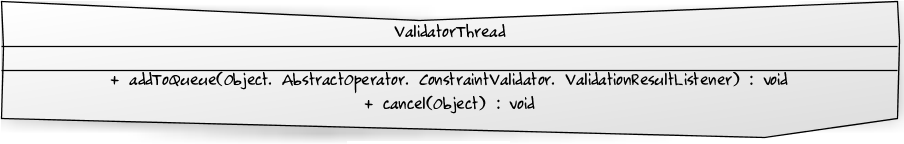
\includegraphics[width=\linewidth]{validatorthread_class} 
  \caption{Class definition of \emph{ValidatorThread}.}
  \label{fig:validatorthread_class}
\end{figure}
Every validation task of a constraint gets enqueued in the \emph{ValidatorThread} after calling the method \emph{addToQueue(...)}.
An identifier is used for each constraint which enables elimination of duplicate tasks for the same constraint in order to minimize the execution time. Tasks can also manually be removed from the queue by calling \emph{cancel(...)}. After a validation task is finished the result is published via callback to the \emph{ValidationResultListener}.









\subsection{External interface of LTLCreator}
\label{sec:easeofintegration}

\emph{LTLCreator} should be integratable into other state machine based programming environments. This is ensured by its implementation as a Java Swing component and a clear API which enables a wide range of use for this tool.

Figure~\ref{fig:coalescence} points out interactions between \emph{LTLCreator} and programming environments it is integrated in.
\begin{figure}[htbp]
  \centering
  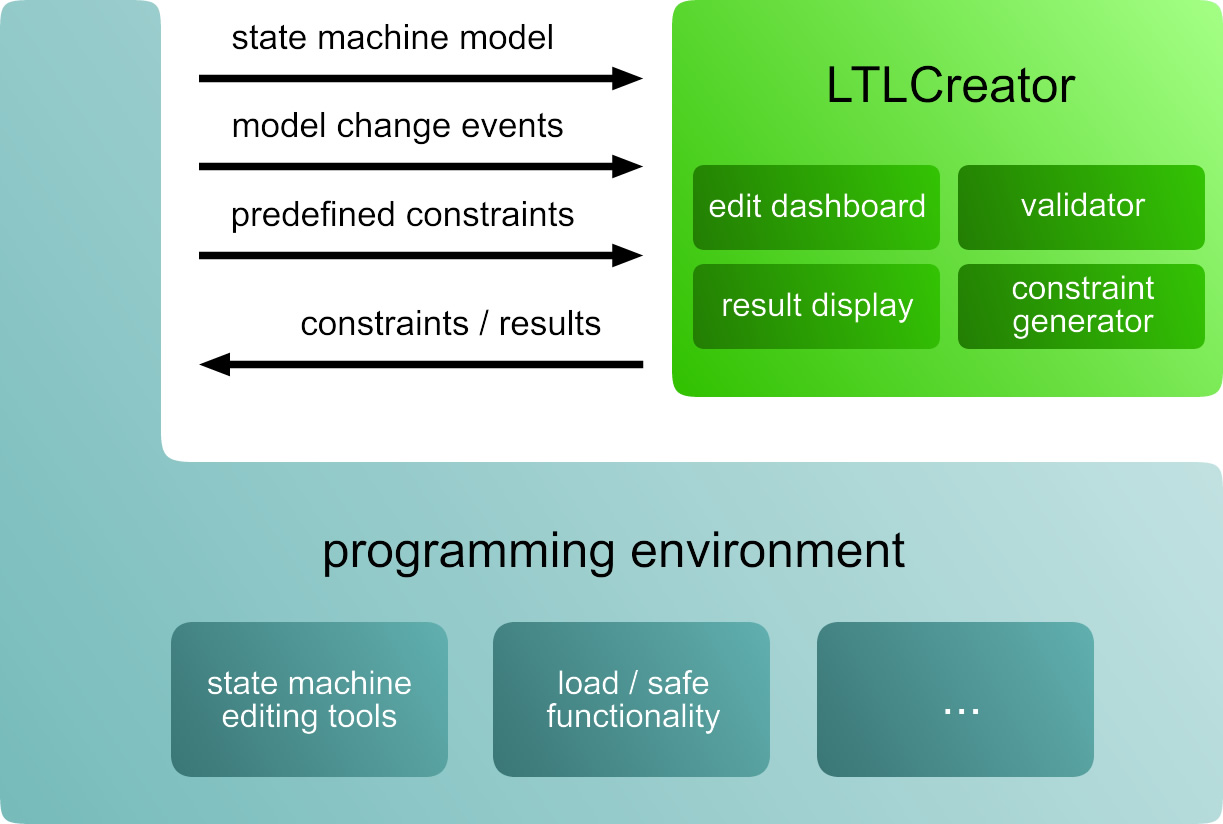
\includegraphics[width=0.7\linewidth]{coalescence}
  \caption{Interaction between LTLCreator and programming environment.}
  \label{fig:coalescence}
\end{figure}
The programming environment provides the state machine model and notifies the \emph{LTLCreator} component about all changes made to the model. This will automatically revalidate all existing constraints and always hold the up-to-date model for constraint generation.
For load and save functionality, all existing constraints can be received and new ones can be added to the \emph{LTLCreator} component programmatically.
All this functionality can be accessed through methods provided by the component \emph{LTLCreator}. Its class definition is shown in figure~\ref{fig:ltlcreator_class}. Whenever there is a change to the state machine, \emph{setModel(Fsm)} has to be called with the current state machine as parameter. This will cause the editor to revalidate where necessary. Constraint exchange can be done by using the methods \emph{addNewDashboard(AbstractOperator, ...)} and \emph{getOperators()}.

\begin{figure}[htbp]
  \centering
  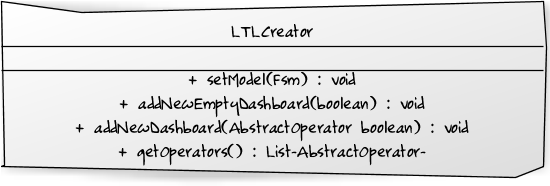
\includegraphics[width=0.65\linewidth]{ltlcreator_class}
  \caption{Class definition for \emph{LTLCreator}.}
  \label{fig:ltlcreator_class}
\end{figure}







\section{Integration into Robostudio}
\label{sec:integrationintorobostudio}

As stated in the previous section, the \emph{LTLCreator} provides an API for integration into other Java based applications. Robostudio,
a visual programming environment for rapid authoring and customization of complex services on a personal service robot, is such an application which was used for evaluating the visual language as well as the automated constraint generation feature and is also supposed to provide all this functionality for development of service robot behaviour in future.

Robostudio uses NetBeans~\cite{netbeans} as a platform and organizes all tools and features in windows. Thus also \emph{LTLCreator} was put into a window and added to the Robostudio platform. This was done by placing it into a NetBeans module which was added to Robostudio's modules. This module imports the \emph{LTLCreator} tool, archived as a jar file, and further consists of only two classes: \emph{LTLCreatorTopComponent} and \emph{XmlDataToLTLEditorDataWrapper}. The former implements the \emph{TopComponent} provided by NetBeans which can be used for displaying UI elements. In order to visualize the \emph{LTLCreator} component it is directly placed on the \emph{LTLCreatorTopComponent}. It retrieves changes of the model and passes them to the \emph{LTLCreator} component. Since the defining of safety constraints is an important issue not only after but also during the process of developing service robot behaviour, the \emph{LTLCreator} window as a vital tool has been positioned in the center of the platform where also the \emph{UI Component Layout Editor Window} is located.
The \emph{XmlDataToLTLEditorDataWrapper} forms the bridge between Robostudio's own model and the state machine model used by \emph{LTLCreator}. All complex data coming from Robostudio has to be cleaned from unimportant layout information and transformed to an elementary state machine representation before it can be processed by \emph{LTLCreator}.



%TODO: load and save



\subsection{Problems}

As already proposed in section~\ref{sec:easeofintegration}, all changes to the state machine program made within Robostudio must of course cause the \emph{LTLCreator} module to revalidate all existing constraints. This demands a concept of change notification management which is responsible for receiving all changes and making this information available for the \emph{LTLCreator} component. As a solution, all parts of the code where model changes are made should be extended with short code snippets which send notifications.
However, this is not as easy to realise in Robostudio since some of the relevant code was generated or even imported as external jars which makes code manipulation impossible.

A second challenge is the current data handling policy in Robostudio. Since this platform is mainly made for developers who used to edit RBDL xml code manually, Robostudio aims for visual rapid editing rather than for syntax checks. Thus syntax errors are not detected or even ignored by static analysis or input restrictions. In fact, such features haven't been requirements for Robostudio. During integration of \emph{LTLCreator} into Robostudio problems came up like transitions leading to non existing states, transitions leading to nowhere (null) or transitions whose target is depending on runtime facts.
This characteristic seems to be a problem for the \emph{LTLCreator} which needs a complete state machine as input and doesn't know how to cope with inconsistent data retrieved from Robostudio.




\subsection{Solutions}

To guarantee that all model changes cause the constraints to be revalidated, all relevant code parts have to report on this. But modification of the code has not been possible in all cases. Whereas all state changes are announced, transition changes stay unnoticed. This decision is sufficient for the prototype, but the developers of Robostudio announced an adapted architecture to solve this problem in the next version.


The problem with inconsistent data could be solved by plausibility and syntax checks during the transformation process of \emph{XmlDataToLTLEditorDataWrapper}. After successful transformation the state machine is passed to the \emph{LTLCreator} component. Otherwise no validation result is displayed for constraints and a dialog lists all identified syntax errors. In the context of safety and reliability a restrictive approach which gives no result at all seemed more applicable than an attempt to interpret the inconsistent data. 